\chapter{The turbulence phenomena}
\label{chap-Turbulence}
One of the main topics of this thesis is the turbulence phenomena that appear in incompressible fluid flows. In order to put the reader in context, it worth describing the main properties and definitions of such kind of flows, albeit rather briefly. 

Some elementary definitions are established in the first section of this chapter. Thereafter, a short introduction to the vorticity is given, together with some characteristic properties of this field. The definition of the Reynolds stresses is stated subsequently, giving some insights of what does \textit{turbulence modelling} mean. In forthcoming chapters, some turbulent quantities will be used to characterize the fluid flow, so we dedicate some lines in this chapter on the explanation of such quantities. Finally, particular characteristics of isotropic turbulence and wall bounded turbulent flows are detailed. Here we introduce the turbulence tests performed during the thesis.

For a deeper explanation of turbulence phenomena we refer to \cite{pope,davidson,orlandi,tennekes,lesieur}.

\section{Introduction to turbulence}
\label{sec-C3_introduction}
\subsection{Elementary concepts}
In the comming chapters some elmentary conceps will be used. Here we give a brief definition of the most important ones:
\begin{itemize}
\item\keyword{Categories of fluid flow:}\\Fluid mechanics and fluid flows are often divided into different regimes. In particular, one can make three different sub-divisions. The first division distinguishes between fluids that may be treated as inviscid or fluids in where the finite viscosity must be taken into account. The second sub-division distingishes between laminar (organized) and turbulent (chaotic) flow. The final sub-division is between irrotational(or potential) flow and rotational flow.

In this thesis we will mainly focus on the second sub-division, distinguishing between laminar and turbulent flows. Except when stated, the fluid will be considered to be viscous and rotational.

\item\keyword{Newton's law of viscosity}\\In most fluids the shear stress is quantified using an empirical law known as Newton's law of viscosity. This law says that a shear stress, $\tau$, is required to cause relative sliding of the fluid layers. Moreover it states that $\tau$ is directly proportional to the angular distortion rate $\frac{d\gamma}{dt}$. It can be shown that in a one-dimensional flow (being $x$ the flow direction), $ u_x(y) $, $ \frac{d\gamma}{dt}=\frac{\partial u}{\partial y} $. Then the shear stress can be writen as
$$\tau=\rho\nu\frac{\partial u_x}{\partial y},\quad\quad\nu=\frac{\mu}{\rho}.$$
Where $ \nu $ is called the kinematic viscosity.

For two-dimensional flow, Newton's law of viscosity becomes
$$ \tau_{xy}=\rho\nu\left(\frac{\partial u_x}{\partial y}+\frac{\partial u_y}{\partial x}\right). $$

%Shear stresses are important not just because they cause fluid elements to distord, but because an imbalance in shear stress can give rise to a net force on individual fluid elements.

\item\keyword{Reynolds number}\\We define the inertial force of a fluid as the force due to the fluid motion and the viscous force as the force produced by the friction. The visous forces per unit volume have a size: $ f_\nu\sim\frac{\rho\nu|\mathbf{u}|}{l_\bot^2} $, where $ l_\bot^2 $ is a characteristic length scale normal to the streamlines. The inertial forces per unit volume are of the order of: $ f_{in}\sim\frac{\rho |\mathbf{u}|^2}{l} $, where $ l $ is a typical geometric lenght scale. 

We can estimate the ratio between the inertial forces and the viscous forces. This ratio is called \textit{Reynolds number},
$$Re=\frac{\frac{\rho |\mathbf{u}|^2}{l}}{\frac{\rho\nu|\mathbf{u}|}{l_\bot^2}}=\frac{ul}{\nu}.$$

When $ Re $ is small, viscous forces outweight inertial forces (laminar regimes), and when $ Re $ is large, viscous forces are relatively small compared against the inertial ones (turbulent regime).

\item\keyword{Boundary layers}\\ Let us consider a high Reynolds number flow. Since $Re$ is large, we might be tempted to solve the inviscid equations of motion, 
$$(\u\cdot\nabla)\u=-\nabla\left(\frac{p}{\rho}\right)$$
subject to the inviscid boundary condition $\u\cdot dS=0$ on all solid surfaces. This determines the so-called \textit{external problem}. If the fluid satisfies the no-slip condition $\mathbf{u}=0$, there must be some region where the velocity adjust to zero. This region is the called \textit{Boundary Layer}. In this region the only mechanical forces available to cause a drop in velocity are viscous shear stresses. Thus the viscous term must be of the same order as the other terms within the boundary layer, 
$$\nu\Delta\u\sim(\u\cdot\nabla)\u,$$

If the inertial forces are of the same order than the viscous forces in the boundary layer, we can stablish the following relation
\begin{eqnarray*}
f_{in}&\sim& f_\nu\\
\frac{\rho u^2}{l} \sim\frac{\rho\nu u}{\delta^2} &\Rightarrow& \frac{\delta}{l}\sim\left(\frac{ul}{\nu}\right)^{-1/2}=Re^{-1/2},
\end{eqnarray*}
being $\delta$ the size of the boundary layer and $l$ the characteristic domain size. Thus we see that, no matter how small we make $\nu$, there is always some boundary layer where shear stresses are important.

Since $Re$ is large, $\delta\ll l.$ When the boundary layer is so thin, the pressure within a boundary layer is virtually the same as the pressure immediately outside the layer.

Boundary layers have another important characteristic, called \textit{separation}, that occurs when the fluid in the boundary layer is ejected into the external flow and a turbulent wake forms. This separation is caused by the pressure forces. When the adverse pressure gradient ($\nabla p>0$) is big enough, the flow in the boundary layer decelerates and reduces the momentum. Then, the fluid in the boundary layer has less momentum than the corresponding external flow and very quickly it comes to a halt, reverses direction and moves off into the external flow, thus forming a wake.

\item\keyword{Laminar and Turbulent flow:}\\It is an empirical observation that at low values of $Re$ flows are laminar, while at high values of $Re$ they are turbulent (chaotic).

A turbulent flow is charactarised by the fact that, superimposed on the mean flow patern, there is random, chaotic motion. The transition from laminar to turbulent flow occurs because, at certain value of $Re$, inestabilities develop in the laminar flow, usually driven by the inertial forces. At low values of $Re$ these potential inestabilities are damped out by viscoity, while at high values of $Re$ the damping is inadequate.

\end{itemize}

\subsection{Vorticity}
%%% REVIEW!!!
The vorticity is a measure of the rotation of individual fluid elements and it is defined by the following expresion
$$\omega\cdot d\mathbf{S}=\oint_C\mathbf{u}\cdot d\mathbf{l}.$$
%%%

Vorticity cannot be created within hte interior of a fluid unless there are body forces present, but it spreats by diffusion and can be intensified by streaching of fluid elements. Boundary layers can be thought as diffusion layers for the vorticity generated on a surface.

Sometimes it is more fruitful to work with the vorticity field instead than the velocity field. First, because the rules governing the evolution of $\omega$ are somewhat simpler than those governign $\u$. The second reason is that many flows are characterized by localised regions of intense rotation. When we are interested in rotation, it is natural to focus on angular momentum rather than linear momentum. Operating with the angular momentum, one can obtain an equation describing the vorticity motion, see \cite{Davidson?}.
\begin{equation}
\label{eq-vorticity}
I\frac{D\omega}{Dt}=-\omega\frac{DI}{Dt}+2\nu\mathbf{T}
\end{equation}
where $I$ is the moment of inertia of a small material element that is \textit{instantaneously} spherical and $\nu\mathbf{T}$ denotes the viscous torque acting on the sphere. The equation \Eq{vorticity} suggest several results:
\begin{itemize}
\item $\omega$ evolves indepently of $ p $.
\item If $\omega$ is initially zero, and the flow is inviscid ($ \nu=0 $), then $\omega$ should remain zero in each fluid particle.
\item If $I$ decreases (the vortex is stretching) in a inviscid fluid element, then the vorticity of that element should increase.
\end{itemize}
Alternatively to \Eq{vorticity}, introducing the identity $\nabla(\u^2/2)=(\u\cdot\nabla)\u+\u\times\omega$ into the linear momentum equation \Eq{...} and operating, we obtain another expression of the vorticity motion in terms of the velocity field
\begin{equation}
\label{eq-vorticity_velocity}
\frac{D\omega}{Dt}=(\omega\cdot\nabla)\mathbf{u}+\nu\Delta\omega.
\end{equation}
From \Eq{vorticity} and \Eq{vorticity_velocity} we can easily see that the rate of rotation of a fluid blob may increase or decrease due to changes in its moment of inertia, or changes because it is spun up or slowed down by viscous stresses. We also can state from equation \Eq{vorticity_velocity} that vorticity is advected by $\u$ and diffused by viscous stresses.

Looking at the equation \Eq{vorticity_velocity} we can see that in three-dimensional flows the first term on the right hand side is non-zero. Comparing this equation with the angular momentum equation \Eq{vorticity}, we can say that $(\omega\cdot\nabla)\u$ represents intensification of vorticity by the streaching fluid elements, a justification of this suggestion can be fount in \cite{Pope}.

\subsection{Reynolds stresses and turbulence models}
It is an empirical observation that if $Re$ is large enough a flow invariably becomes unstable and then turbulent. Suppose we have a turbulent flow in which $\u$ and $p$ consist of a time-averaged component, $\overline{\u}$ and $\overline{p}$, plus a fluctuating part, $\u'$ and $p'$:
$$\u=\overline{\u}+\u',\qquad p=\overline{p}+p'.$$
Taking the $x$-component of the time averaged equation of motion we have that
\begin{eqnarray}
\label{eq-momentum_x}
(\overline{\mathbf{u}}\cdot\nabla)\overline{u}_x=-\frac{\partial}{\partial x}\left(\frac{p}{\rho}\right)+\frac{\partial}{\partial x}\left[2\nu\frac{\partial \overline{u}_x}{\partial x}\right]+\frac{\partial}{\partial y}\left[\nu\left(\frac{\partial \overline{u}_x}{\partial y}+\frac{\partial \overline{u}_y}{\partial x}\right)\right]+\\ \nonumber
+\frac{\partial}{\partial z}\left[\nu\left(\frac{\partial \overline{u}_x}{\partial z}+\frac{\partial \overline{u}_z}{\partial x}\right)\right]+\frac{\partial}{\partial x}[-\overline{u_x'u_x'}]+\frac{\partial}{\partial y}[-\overline{u_x'u_y'}]+\frac{\partial}{\partial z}[-\overline{u_x'u_z'}].
\end{eqnarray}
We determine the laminar stresses from the Newton's law of viscosity, taking into account only the time-averaged components
\begin{eqnarray*}
\sigma_x&=&2\rho\nu\frac{\partial \overline{u}_x}{\partial x},\\
\tau_{xy}&=&\rho\nu\left[\frac{\partial \overline{u}_x}{\partial y}+\frac{\partial \overline{u}_y}{\partial x}\right],\\
\tau_{xz}&=&\rho\nu\left[\frac{\partial \overline{u}_x}{\partial z}+\frac{\partial \overline{u}_z}{\partial z}\right].
\end{eqnarray*}
From \Eq{momentum_x} we see that the turbulent flow have additional stresses that are not considered on the laminar definition. These stresses are called \textit{Reynolds stresses} and are determined by
\begin{eqnarray*}
\sigma_x^R&=&-\rho\overline{u_x'u_x'},\\
\tau_{xy}^R&=&-\rho\overline{u_x'u_y'},\\
\tau_{xz}^R&=&-\rho\overline{u_x'u_z'}.
\end{eqnarray*}
Then, we can rewrite \Eq{momentum_x} in a more compact way:
\begin{equation}
\label{eq-momentum_x_reynolds}
\frac{\partial \bar{u}_x}{\partial t}+(\bar{\mathbf{u}}\cdot\nabla)\bar{u}_x=-\frac{\partial\bar{p}}{\partial x}+\nu\nabla^2\bar{u}_x+(\nabla\cdot\T)_x,
\end{equation}
being
$$\T=\left[\begin{array}{ccc}
\sigma_x^R&\tau_{xy}^R&\tau_{xz}^R\\
\tau_{yx}^R&\sigma_y^R&\tau_{yz}^R\\
\tau_{zx}^R&\tau_{zy}^R&\sigma_z^R
\end{array}\right]$$
the Reynolds stress tensor. If we wish to make predictions from equation \Eq{momentum_x_reynolds} we need to be able to relate the Reynolds stresses, $ -\rho\overline{u_x'u_i'} $, to some quantity which we know about, such as mean velocity gradients of the type $ \frac{\partial\overline{u}_x}{\partial y} $. This is the purpose of \textit{turbulence modelling}. In effect, a turbulence model provides a means of estimating Reynolds stresses.

\subsubsection{The Closure Problem of Turbulence}
In a turbulent fluid, $\u$ is a chaotic field and vary from one realization of a flow to the next. But the statistical properties of $\u$ seem to be well behaved and perfectly reproducible. It turns out to be possible to manipulate the Navier-Stokes equations into a hierarchy of statistical equations of the form, 
$$\frac{\partial}{\partial t}[\mbox{certain statistical properties of }\mathbf{u}]=f(\mbox{other statistical properties of }\mathbf{u}).$$

It can be shown that this system of equations is not closed, in the sense that, no matter how many manipulations we perform, there are always more statistical unknowns than equations relating them. This is known as the \textit{closure problem of turbulence}, and it arises because of the non-linearity of the Navier-Stokes equations.

\subsubsection{Reynolds stresses decomposition}
\label{subsubsec:reynolds_decomposition}
Leonard (1974) introduced a decomposition of $\tau_{ij}^R$ into three component stresses.
$$\tau_{ij}^R=L_{ij}+C_{ij}+R_{ij},$$
where $L_{ij}=\overline{\overline{u}_i\overline{u}_j}-\overline{u}_i\overline{u}_j$ are the Leonard stresses. The cross stresses are $C_{ij}=\overline{\overline{u}_iu_j'}+\overline{u_i'\overline{u}_j}$ and finally, $R_{ij}=\overline{u_i'u_j'}$ are the subgrid scale (SGS) Reynolds stresses. Decomposing Reynolds stresses into Leonard, cross and SGS Reynolds stresses we can reformulate \Eq{momentum} as
$$\frac{\partial \overline{\u}}{\partial t}+(\overline{\u}\cdot\nabla)\overline{\u}=-\frac{\partial\overline{p}}{\partial x}+\nu\nabla^2\overline{\u}+\nabla\cdot\L+\nabla\cdot\C+\nabla\cdot\Rbb$$

\subsection{Definition of some turbulent quantities}
Turbulent flows are considered to be cahotic since, superimposed on the mean flow patern, there appear a fluctuating and random, both in space and time, motion. In general, the simulation of this kind of flows requires a large amount of computational resources. This occurs because the size of spatial and temporal scales needed to accurately reproduce the flow are extremly fine. In order to simplify the simulation, instead of resolving all fluid flow scales, we can simulate the mean flow patern, \textit{i.e.} the largest scales, which in most engineering problems is enough, and consider how the unresolved scales interact with the largest ones taking into account their gross statistical properties. Then, if we want to ensure that the simulation reflects the correct mean flow and the effect of the small scales on the larges is accurately predicted we need some verification tools. These tools are some turbulent quantities that we can evaluate in our simulation and with which we can compare with analytical or more accurate results. In general, these quantities are obtained through an averaging procedure of the fluctuating fluid motion. We define the averaging procedure for a generic quantity $q$ as
$$\left\langle q\right\rangle=\frac{1}{\Pi_{i=1}^{n_d}N_i}\sum_{j_1,...,j_{n_d}}q_{j_1,...,j_{n_d}},$$
that is averaged over $n_d$ dimensions, each dimension $i$ having $N_i$ evaluation points. 

In this section we will briefly define the turbulent quantities that are going to be used to characterize the turbulent flow simulations and that will allow us to compare the results againts the references. We can find a more complete definition of the turbulent quantities that are going to be stated in this section in \cite{orlandi,pope,davidson}.

\begin{itemize}
\item\keyword{Velocity correlation function}\\ The velocity correlation function is defined by
\begin{equation}
\label{eq-velocity_correlation}
Q_{ij}=\left\langle u_i'(\x)u_j'(\x+\r)\right\rangle.
\end{equation}
In general $Q_{ij}$ also depends on time. $Q_{ij}$ tells us about the degree to which, and the manner in which, the velocity components at different points are correlated to each other. However, the velocity correlation function does not, in of itself, tell us how the kinetic energy is distributed across the different eddy sizes. Rather, we must introduce two additional quantities like the second-order structure function and the energy spectrum.
\item\keyword{Second-order structure function}\\ The second-order longitudinal structure function is defined in terms of the longitudinal velocity increment, $\Delta u(r)=u_x(\x+r\hat{\e}_x)-u_x(\x)$, as follows:
\begin{equation}
\label{eq-second_order_structure}
\left\langle[\Delta u(r)]^2\right\rangle=\left\langle[u_x(\x+r\hat{\e}_x)-u_x(\x)]^2\right\rangle.
\end{equation}
Only eddies of size $\sim r$, or less, can make significant contribution to $\Delta u$, and so $\left\langle[\Delta u]^2\right\rangle$ is often taken as an indication of the energy per unit mass contained in the eddies of size $r$ or less. 
\item\keyword{Energy spectrum}\\ To determine the distribution of the kinetic energy among the eddies of different size we look at the energy spectrum function $E(k)$. Working with wave number, $k$, we define the energy spectrum via the transform pair
\begin{align}
\label{eq-energy_spectrum}
E(k)=\frac{2}{\pi}\int_0^\infty R(r)kr\sin(kr)dr,\\
\label{eq-autocovariance}
R(r)=\int_0^\infty E(k)\frac{\sin(kr)}{kr}dk.
\end{align}
Where $R(r)=\frac{1}{2}\left\langle\u(\x)\cdot\u(\x+\r)\right\rangle=u^2(g+f/2)$ is called the autocovariance function. The functions $f$ and $g$ are called the longitudinal and lateral velocity correlation coefficients and satisfy the relation $2rg=(r^2f)'$.

In Appendix \ref{appendix-spectrum_implementation}, some tips for the implementation of the energy spectrum calculation are given.
\item\keyword{Total kinetic energy}\\ Taking the limit $r\rightarrow 0$, the equation \Eq{autocovariance} leads to
\begin{equation}
\label{eq-total_kinetic_energy}
R(0)=\frac{1}{2}\left\langle\u^2\right\rangle=\int_0^\infty E(k)dk,
\end{equation}
which is nothing else than the total kinetic energy, $K:=\frac{1}{2}\left\langle\u^2\right\rangle$. Equation \Eq{total_kinetic_energy} tells us that $E(k)dk$ is the contribution to $K$ from all eddies with wave numbers in the range $k\rightarrow k+dk$, where $k\sim\pi/r$. In fact, it is not true at all, but it works if we are on the range $\eta^{-1}<k<l^{-1}$, being $\eta$ and $l$ the Kolmogorov and integral length scales, respectively, defined in following points.
\item\keyword{Enstrophy}\\ The energy spectrum $E(k)$ has one further property
\begin{equation}
\label{eq-enstrophy}
\left\langle\boldsymbol{\omega}^2\right\rangle=\int_0^\infty k^2E(k)dk.
\end{equation}
If we define the enstrophy as $Z:=\frac{1}{2}\left\langle\boldsymbol{\omega}^2\right\rangle$, from \Eq{enstrophy}, the quantity $k^2E(k)$ is interpreted as the contribution to the enstrophy from the range of wave numbers $k\rightarrow k+dk$.
\item\keyword{Skewness factor}\\ The third-order longitudinal structure function is defined, like the second-order longitudinal structure function, as
\begin{equation*}
\label{eq-third_order_structure}
\left\langle[\Delta u(r)]^3\right\rangle=\left\langle[u_x(\x+r\hat{\e}_x)-u_x(\x)]^3\right\rangle.
\end{equation*}
For further discussions, it is more usefull to work with the skewness factor. This factor is a normalized version of the third-order structure function
\begin{equation}
\label{eq-skewness_factor}
S(r)=\frac{\left\langle[\Delta u(r)]^3\right\rangle}{\left\langle[\Delta u(r)]^2\right\rangle^{3/2}}.
\end{equation}
The skewness factor for a decaying turbulent flow depends slightly on the Reynolds number, but usually has a value of around $-0,4\pm0,1$ for $r\rightarrow0$ for $Re$ up to $10^6$, and decays slowly with $r$.
\item\keyword{Root mean square of the velocity field}\\ For a three-dimensional flow, the root mean square (RMS) of the velocity field is given by
$$u=\left(\frac{2}{3}\int_0^\infty E(k)dk\right)^{1/2}.$$
\item\keyword{Kolmogorov scale}\\The viscous dissipation acts most efficiently at small scales. Then, for wavenumbers greater than certain wavenumber $k_\eta$, the viscous dissipation will become important, and the energy spectrum $E(k)$ will decay more rapidly than the inertial range. It can be shown that $$k_\eta\sim\left(\frac{\varepsilon}{\nu^3}\right)^{1/4},$$ with $\varepsilon$ the total energy dissipation rate. The Kolmogorov scale is the inverse of this wave number $\eta:=1/k_\eta$, then $$\eta\sim\left(\nu^3/\varepsilon\right)^{1/4}.$$
\item\keyword{Integral length scale}\\The integral length scale is the scale of the energy-containing eddies. From the Kolmogorov spectrum \Eq{kolmogorov_spectrum} we can determine the wavenumber that defines this scale, $k_\ell$, in terms of the energy dissipation rate  $$k_\ell\sim\frac{\varepsilon}{u^3}.$$ Then, the integral length scale, $\ell$, will be $\ell\sim u^3/\varepsilon$. Taking the ratio between the integral and Kolmogorov scales we have that
$$\frac{\ell}{\eta}\sim\frac{u^3}{\varepsilon^{3/4}\nu^{3/4}}\sim\left(\frac{u\ell}{\nu}\right)^{3/4}\sim Re_\ell^{3/4}.$$
Where $Re_l$ is the integral Reynolds number. Thus, the inertial range includes a set of scales growing with $Re_\ell^{3/4}$. If we want to accurately simulate the inertial range, the number grid points on an uniform 3D mesh should be $N\sim\left((Re_\ell)^{3/4}\right)^3=(Re_\ell)^{9/4}$. 
\item\keyword{Taylor microscale}\\Apart from the Kolmogorov and integral length scale, there is another length scale that can characterize a turbulent flow. This is the Taylor microscale and provides a convenient estimate for the fluctuating strain rate field. It is a standard turbulent length that identifies the inertial subrange. The Taylor microscale is defined as $$\lambda^2=\frac{15u^2}{\left\langle\boldsymbol{\omega}^2\right\rangle}=\frac{15\nu u^2}{\varepsilon}.$$
\item\keyword{Taylor-microscale Reynolds number}\\The Taylor-microscale Reynolds number is associated to the characteristic Taylor-microscale length and it is defined as $$Re_\lambda=\frac{u\lambda}{\nu}=\sqrt{15}\frac{u^2}{\left(\nu\varepsilon\right)^{1/2}}=\frac{1}{\nu}\sqrt{\frac{20}{3}}\frac{\int_0^\infty E(k)dk}{\left(\int_0^\infty k^2E(k)dk\right)^{1/2}}.$$
\item\keyword{Energy dissipation rate}\\For a closed domain wiht stationary boundaries, the total rate of energy dissipation per unit of mass is given by
$$\varepsilon=2\nu\frac{1}{2}\left\langle\boldsymbol{\omega}^2\right\rangle=\frac{15\nu u^2}{\lambda^2}.$$
See Section \ref{subsec-isotropic_energy_dissipation}, where we derive this result.
\end{itemize}

\section{Isotropic turbulence}
\label{sec-C3_isotropic_turbulence}
We understand by isotropic turbulent flow the one in which there is no mean flow and the rotation is negligible. In this situation we do not have any phenomena that introduce anisotropy into the flow. On the other hand, we say that a flow is homogeneous if the spatial gradients of any averaged quantity are negligible. This condition means that the turbulent flow statistics do not depend on space.

\subsection{Energy dissipation}
\label{subsec-isotropic_energy_dissipation}
By definition of homogeneity and isotropy, the velocity mean on the spatial domain is zero. Then, we have to characterize the 3D isotropic turbulent flows relying on the second order statistics of the velocity field, which is nothing else than the kinetic energy, $K=\frac{1}{2}\left\langle\u^2\right\rangle$.

Multiplying the momentum equation \Eq{NS_strong_momentum} by the velocity, assuming that $\f=0$, and operating we have that
\begin{equation}
\label{eq-energy_equation}
\frac{\partial\left(\u^2/2\right)}{\partial t}=-\nabla\cdot\left[\left(\u^2/2\right)\u\right]-\nabla\cdot\left[\left(p\right)\u\right]+\nabla\cdot\left[\left(\nu(\boldomega\times\u)\right)\right]-\nu\boldomega^2.
\end{equation}
Noting that $\frac{\u^2}{2}$ is nothing else than the kinetic energy, equation \Eq{energy_equation} is giving information about how the kinetic energy is dissipated. If we integrate \Eq{energy_equation} over an arbitrary and fixed volume $V$, and using the divergence theorem, we can determine through which mechanisms the energy is dissipating
\begin{align}
\label{eq-energy_dissipation}
&\frac{d}{dt}\int_V\left(\u^2/2\right)dV=\\\nonumber
&-\left[\mbox{rate at which kinetic energy is convected across the boundary}\right]\\\nonumber
&+\left[\mbox{rate at which the pressure forces do work on the boundary}\right]\\\nonumber
&+\left[\mbox{rate at which the viscous forces do work on the boundary}\right]\\\nonumber
&-\int_V\nu\boldomega^2dV.
\end{align}
Averaging \Eq{energy_dissipation} and assuming that for homogeneous and isotropic turbulence the average flux through the boundaries is negligible, we obtain a relation between the averaged total kinetic energy $K$ with the enstrophy $Z$.
\begin{equation}
\label{eq-energy_enstrophy}
\frac{d K}{dt}=-2\nu Z,
\end{equation}
which states that the rate of change of turbulent kinetic energy per unit mass is balanced by the rate of dissipation of mechanical energy per unit mass, $\varepsilon:=2\nu Z=\nu\langle\boldomega^2\rangle$.

\subsection{Kinetic energy in spectral space}
\label{subsec-isotropic_kinetic_energy_spectral}
One may be interested on how the energy is transferred between different scales, which is described by the energy spectrum evolution.

In order to obtain an evolutionary equation for the energy spectrum $E(k,t)$, we will first transform the Navier-Stokes equations \Eq{NS_strong_momentum}-\Eq{NS_strong_continuity} into the Fourier space. Let us consider the integral Fourier representation of the velocity field
$$\hat{\u}(\k,t)=\left(\frac{1}{2\pi}\right)^3\int\exp(-i\k\cdot\x)\u(\x,t)d\x.$$
Under this notation, the incompressibility constrain \Eq{NS_strong_continuity} would read
$$\k\cdot\hat{\u}(\k,t)=0,$$
meaning that the Fourier velocity field $\hat{\u}$ is perpendicular to $\k$. Then, the time derivative $\partial\hat{\u}/\partial t$ and the viscosity term $\nu k^2\hat{\u}$ also belong to the plane perpendicular to $\k$, being $k^2=\sum_{i=1}^dk_i^2$. The pressure gradient is given by $i\hat{p}\k$, which is parallel to the wavevector $\k$. Thus, the Fourier transform of $\u\cdot\nabla\u+\nabla p$ is nothing else than the projection into the plane perpendicular to $\k$ of $\u\cdot\nabla\u$. The final expression of the Navier-Stokes equations in the Fourier space is given by
\begin{equation}
\label{eq-NS_strong_fourier}
\left(\frac{\partial}{\partial t}+\nu k^2\right)\hat{u}_i(\k,t)=-i\int_{\mathbf{p}+\mathbf{q}=\k}q_j\left(\delta_{i,m}-\frac{k_ip_m}{k^2}\right)\hat{u}_j(\mathbf{p},t)\hat{u}_m(\mathbf{q},t)d\mathbf{p}d\mathbf{q}.
\end{equation}
Multiplying \Eq{NS_strong_fourier} by the complex conjugate $\hat{\u}_i^*(\k,t)$ integrating over $\k$, and operating we have that for isotropic turbulence the energy spectrum follows
\begin{equation}
\label{eq-energy_fourier}
\frac{\partial}{\partial t}E(k,t)=T(k,t)-2\nu k^2E(k,t).
\end{equation}
with $T(k,t)$ the term that comprises all triad interaction terms. Integrating over all $k$, and using the relation between the kinetic energy and the total energy dissipation rate given by \Eq{energy_enstrophy} we have that
$$\int_0^\infty T(k,t)dk=0,$$
which means that the nonlinear interactions transfer energy between different wave numbers, but do not change the total energy.

\subsubsection{Kolmogorov spectrum}
\label{subsubsec-Kolmogorov_spectrum}
\begin{equation}
\label{eq-kolmogorov_spectrum}
E(k)\sim C\varepsilon^{2/3}k^{-5/3}.
\end{equation}

\subsection{Benchmark tests}
\label{subsec-isotropic_tests}

\subsubsection{Decay of homogeneous isotropic turbulence}
The Decay of Homogeneous Isotropic Turbulence (DHIT) test is one of the most used benchmarks to test the simulation accuracy of isotropic turbulent flows. Here we want to analyse the statistics of an homogeneous isotropic turbulent flow in a 3D box of size $\Omega=\left\{(0,2\pi)\times(0,2\pi)\times(0,2\pi)\right\}$. The flow is initialized with an initial condition that has a predetermined energy spectrum, considering all the boundary conditions to be periodic.

In this work, we have taken the energy spectrum expression from Mansour \& Wray \cite{mansour_decay_1994}.
\begin{equation}
\label{eq-DHIT_init_spectrum}
E(k,0)=\frac{q^2}{2A}k_0^{-(\sigma+1)}k^4\exp\left(-\frac{\sigma}{2}\left(\frac{k}{k_0}\right)^2\right),
\end{equation}
with $k_0$ the wavenumber at which $E(k,0)$ is maximum, $\frac{q^2}{2}                                                                                                                                                                                                                  $ the total kinetic energy and $A=\int_0^\infty k^\sigma\exp(-\sigma k^2/2)$. In this thesis we choose $q^2=3$ and $\sigma=4$.

With this setting, it can be shown that $A=\frac{3}{32}\sqrt{\frac{\pi}{2}}$. So, the initial energy spectra will be
\begin{equation}
\label{eq-DHIT_init_spectrum2}
E(k,0)=16\sqrt{\frac{2}{\pi}}k_0^{-5}k^4\exp\left(-2\left(\frac{k}{k_0}\right)^2\right).
\end{equation}

Going further, from the definitions of the total kinetic energy ,$K$, and the enstrophy, $Z$, given in \Eq{total_kinetic_energy} and \Eq{enstrophy}, respectively, we can evaluate the initial value of these properties. Hence, we have
\begin{align}
\label{eq-DHIT_intial_K}
K&=\int_0^\infty E(k,0)dk\\\nonumber
&=16\sqrt{\frac{2}{\pi}}k_0^{-5}\left(-\frac{k_0^2}{4}\right)\int_0^\infty k^3\left(-\frac{4k}{k_0^2}\right)\exp\left(-2\left(\frac{k}{k_0}\right)^2\right)dk\\\nonumber
&=12\sqrt{\frac{2}{\pi}}k_0^{-3}\left(-\frac{k_0^2}{4}\right)\int_0^\infty k\left(-\frac{4k}{k_0^2}\right)\exp\left(-2\left(\frac{k}{k_0}\right)^2\right)dk\\\nonumber
&=3\sqrt{\frac{2}{\pi}}k_0^{-1}\left(\frac{k_0}{\sqrt{2}}\right)\int_0^\infty\left(\frac{\sqrt{2}}{k_0}\right)\exp\left(-2\left(\frac{k}{k_0}\right)^2\right)dk\\\nonumber
&=3\sqrt{\frac{2}{\pi}}k_0^{-1}\left(\frac{k_0}{\sqrt{2}}\right)\frac{\sqrt{2}}{2}\\\nonumber
&=\frac{3}{2},
\end{align}
and
\begin{align}
\label{eq-DHIT_inital_Z}
Z&=\int_0^\infty k^2E(k,0)dk\\\nonumber
&=16\sqrt{\frac{2}{\pi}}k_0^{-5}\left(-\frac{k_0^2}{4}\right)\int_0^\infty k^5\left(-\frac{4k}{k_0^2}\right)\exp\left(-2\left(\frac{k}{k_0}\right)^2\right)dk\\\nonumber
&=20\sqrt{\frac{2}{\pi}}k_0^{-3}\int_0^\infty k^4\exp\left(-2\left(\frac{k}{k_0}\right)^2\right)dk\\\nonumber
&=\frac{5}{4}k_0^2\int_0^\infty E(k,0)dk\\\nonumber
&=\frac{15}{8}k_0^2.
\end{align}

Following Rogallo \cite{rogallo_numerical_1981}, we generate the initial field on the Fourier space such that it satisfies continuity and has the energy spectrum prescribed in (\ref{4.2.1}). First, we define two complex parameters:
$$\alpha=\left(\frac{E(k,0)}{2\pi k^2}\right)^{1/2}\exp(i\theta_1)\cos(\phi),$$
$$\beta=\left(\frac{E(k,0)}{2\pi k^2}\right)^{1/2}\exp(i\theta_2)\cos(\phi).$$

Where $\theta_1$, $\theta_2$ and $\phi$ are random numbers on the interval $(0,2\pi)$. With $\alpha$ and $\beta$ we can construct a solenoidal field in the wave number space whose initial spectrum is equal to $E(k,0)$.
\begin{align}
\label{eq-DHIT_initial_u_fourier}
\hat{u_1}=(\alpha|k|k_2+\beta k_1k_3)/(|k|k_h),\\\nonumber
\hat{u_2}=(-\alpha|k|k_2+\beta k_3k_2)/(|k|k_h),\\\nonumber
\hat{u_3}=(-\beta k_h^2)/(|k|k_h),
\end{align}
where $k_h=\left(k_1^2+k_2^2\right)^{1/2}$ and $|k|=\left(k_1^2+k_2^2+k_3^2\right)^{1/2}$.

To have the field \Eq{DHIT_initial_u_fourier} in the physical space we apply the inverse Fast Fourier Transform, see Appendix \ref{appendix-spectrum_implementation} for a detailed description of the implementation fo the Fourier Transform.

In order to check the accuracy of the proposed methods, we will compare the results with those showed in \cite{_selection_????}. Then, we set $k_0=6$ and the viscosity such that the asossiated Taylor-microscale Reynolds number is $Re_\lambda=952$,
$$Re_\lambda=\sqrt{\frac{20}{3}}\frac{\int_0^\infty E(k)dk}{\nu\left(2\int_0^\infty k^2E(k)dk\right)^{1/2}}=952\,$$
which results in $\nu=3.5014006\cdot 10^{-4}$.

In \Fig{DHIT_initial_spectrum} we show the initial analytical energy spectrum and the one calculated from the initial velocity field on the Fourier space \Eq{DHIT_initial_u_fourier} using a $128^3$ linear elements mesh. We observe that the computed energy spectrum is equivalent to the analytical one, a fact that we were expecting since we use the initial field proposed by Rogallo \cite{rogallo_numerical_1981}, which precisely satisfies this condition.
\begin{figure}[h!]
	\centering	
	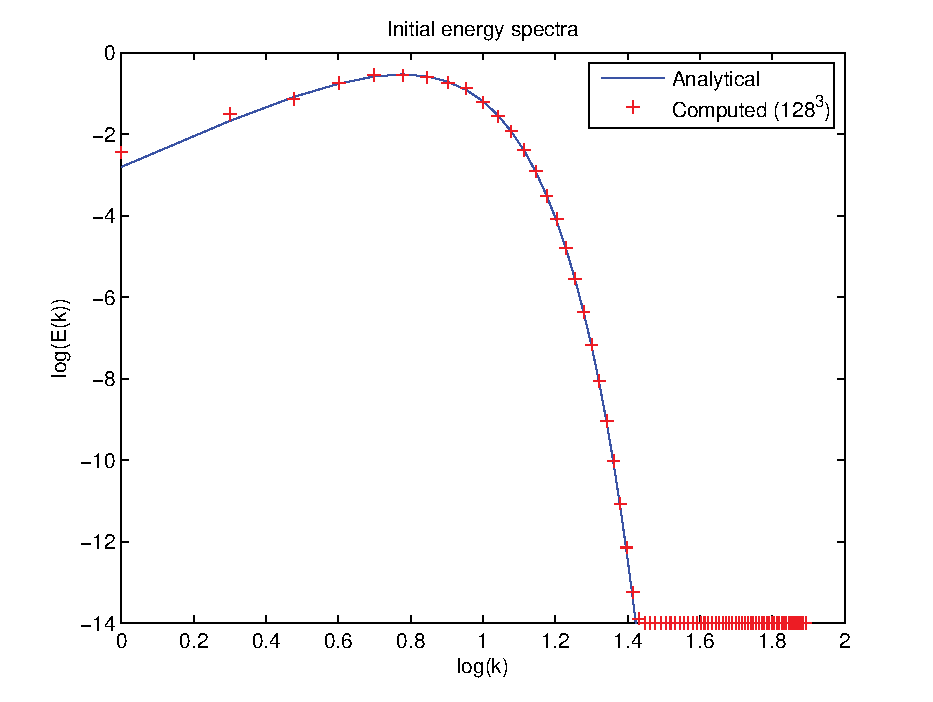
\includegraphics[width=0.6\textwidth]{Figures/Chapter3/DHIT_initial_energy}
	\caption{Analytical and computed initial energy spectrum for the DHIT test.}
	\label{fig-DHIT_initial_spectrum}
\end{figure}

In \Fig{DHIT_isovorticity} we depict the characteristic structures of a fully developed homogeneous and isotropic turbulent flow, plotting the vorticity isosurfaces obtained in the DHIT tes.
\begin{figure}[h!]
	\centering	
	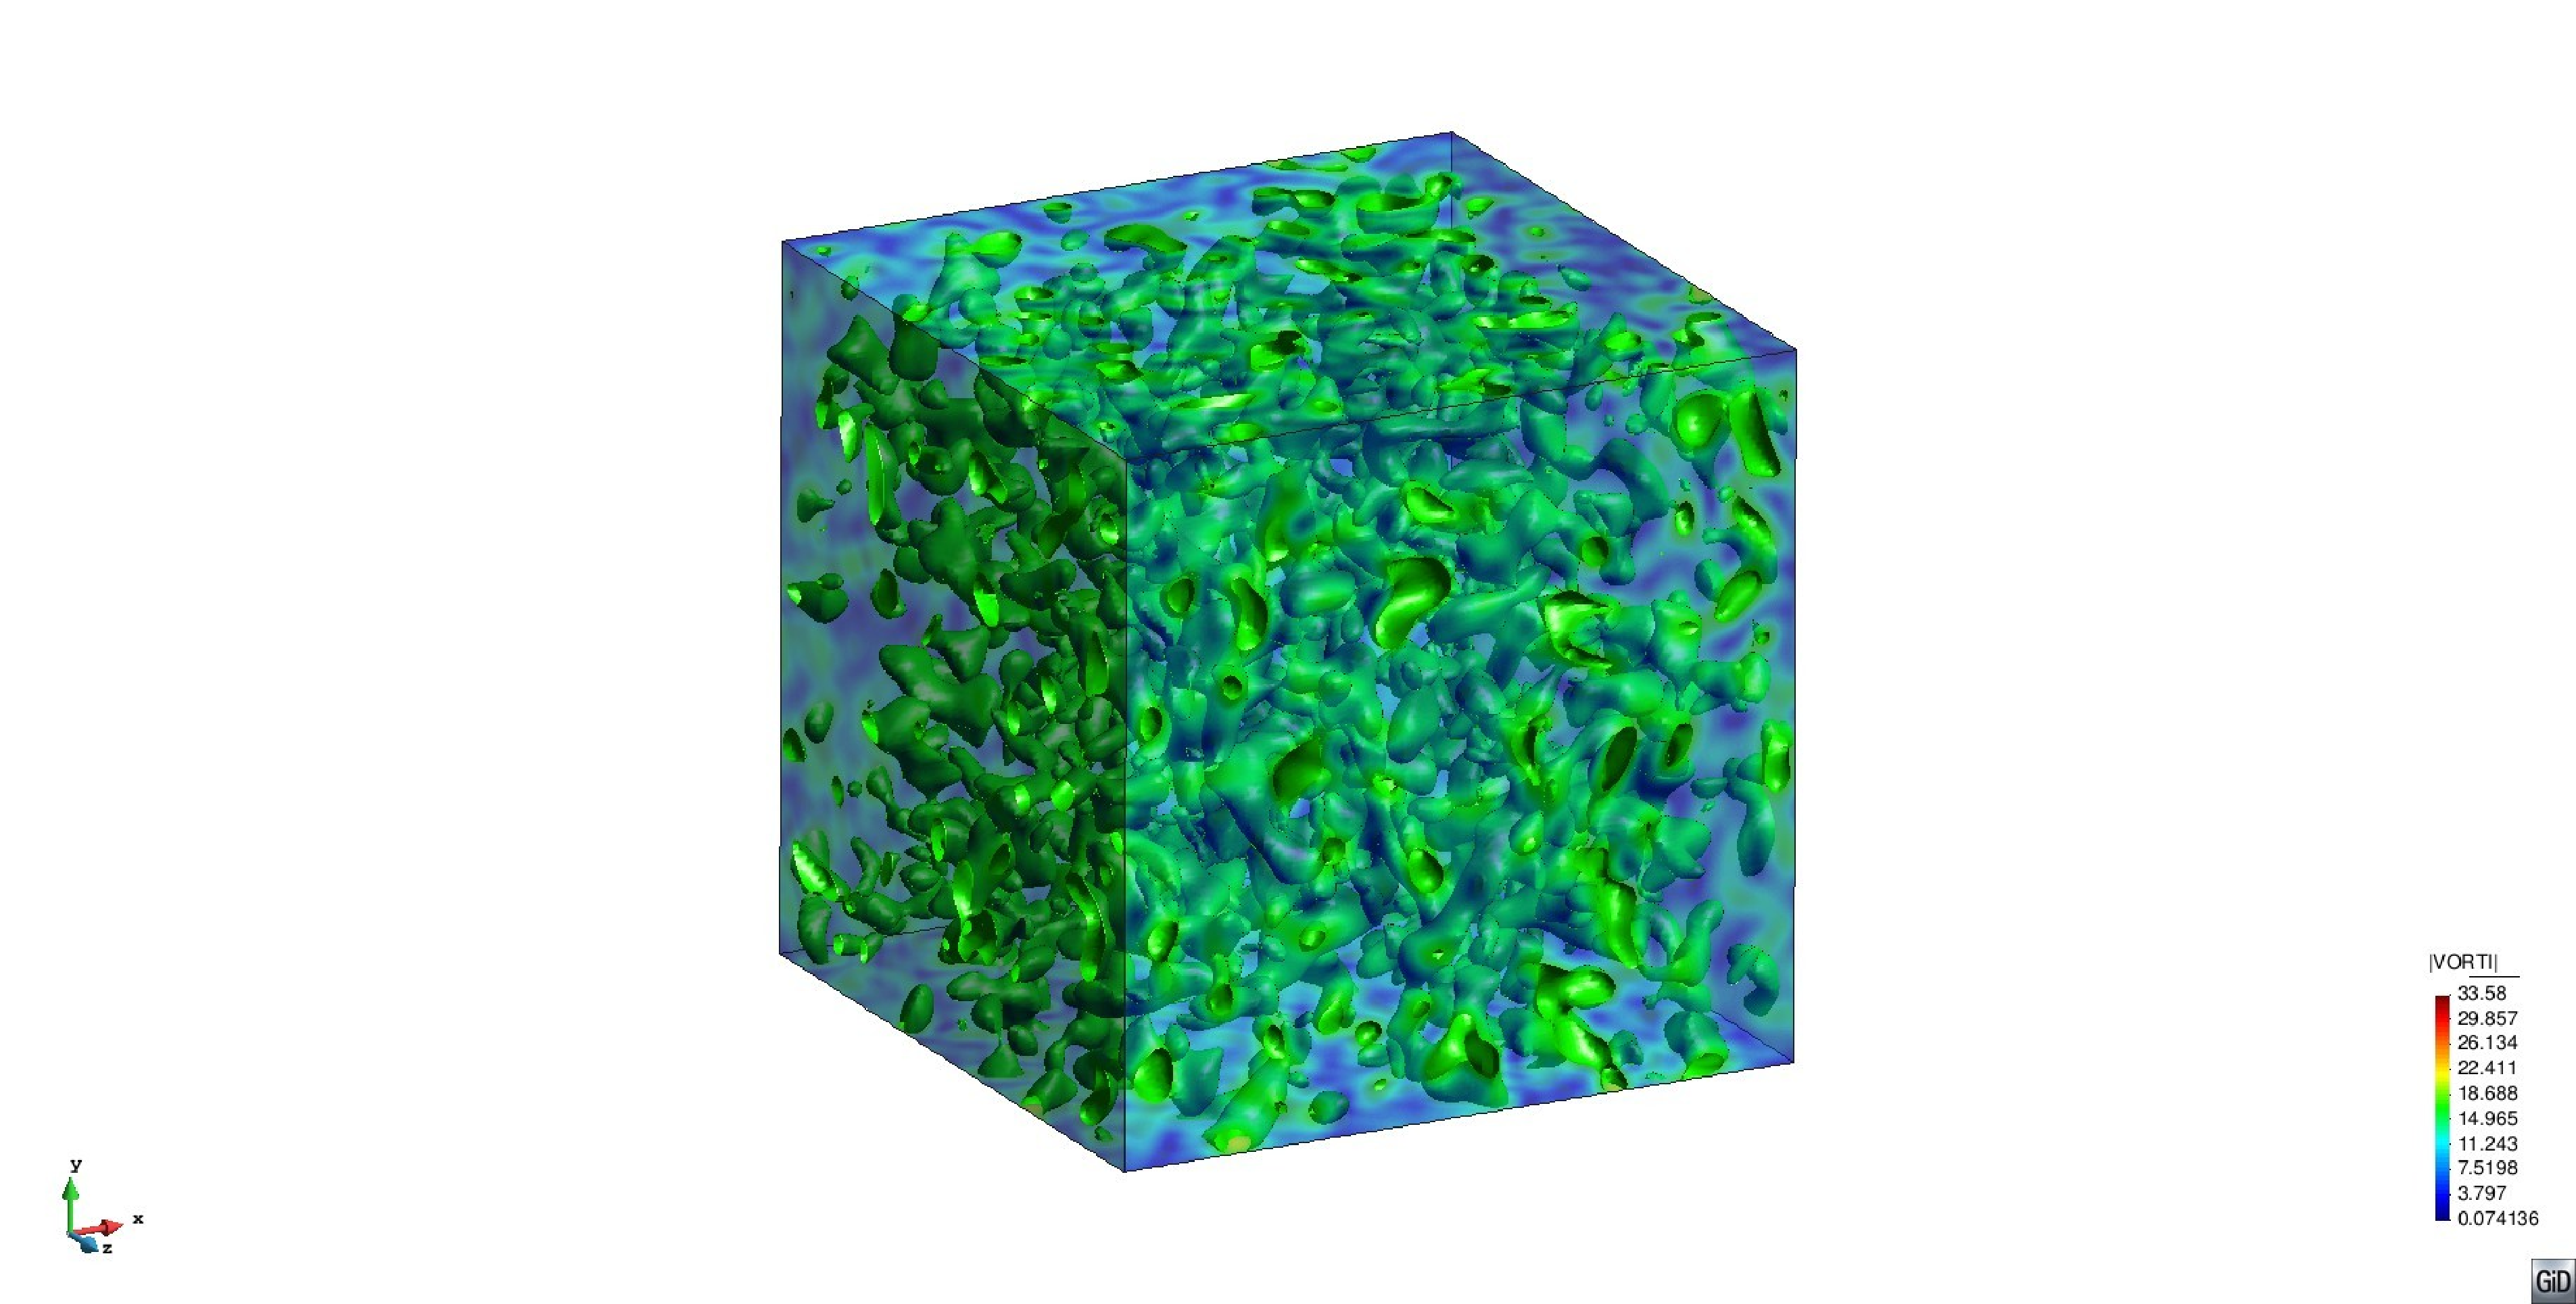
\includegraphics[trim=18cm 3.3cm 14cm 3.2cm,clip=true,width=0.7\textwidth]{Figures/Chapter3/DHIT_isovorticity}
	\caption{Vorticity isosurfaces in the DHIT test.}
	\label{fig-DHIT_isovorticity}
\end{figure}

The initial condition has a relevant role on homogeneous isotropic turbulence. In the final periods of decay, as has been exposed by \cite{hinze_turbulence_1975}, the energy spectrum follows the linear decay law,
\begin{equation}
\label{eq-DHIT_final_decay}
E(k,t)=E(k,0)\exp(-2\nu k^2t).
\end{equation}
So, a first conclusion we can point out from \Eq{DHIT_final_decay} is that the initial spectra, $E(k,0)$, in the final period of decay, has a direct relation with the decay exponent. The total kinetic energy can be calculated integrating \Eq{DHIT_final_decay} over all wave numbers. Then, when $t\rightarrow\infty$, the power law decay is determined by the shape of the initial spectrum.

Moreover, \cite{Staffman 1967} showed that if the initial field is generated by random impulsive forces, a spectrum of the form
\begin{equation}
\label{eq-DHIT_staffman_decay}
E(k,t)\sim k^2\exp(-2\nu k^2t)
\end{equation}
will ensue. Then, the total kinetic energy will decay with the law $K\sim t^{-3/2}$. But, anyway, we will not consider the case of having impulsive forces acting on the flow.

Also in this direction \cite{rohe_analysis_2010} and \cite{chalot_consistent_1998}, say that in the long-run, the energy should decay following the $t^{-1.4}$ law.

\subsubsection{Taylor-Green Vortex flow}
The Taylor-Green Vortex flow (TGV) problem is also a typical and widely used problem on turbulence numerical simulations. First introduced by Taylor and Green (1937) \cite{taylor}, this problem aims to show, in a relatively simple flow, the basic turbulence decay mechanisms like the turbulent energy cascade, the production of small eddies and the enhancement of dissipation by the stretching of vortex lines.

The initial analytical condition for this problem, unlike the DHIT problem, is defined on the physical space. Here we follow \cite{gassner_accuracy_????}, where the initial solution is defined by
\begin{align}
\label{eq-TGV_initial_condition}
&u_x=u_0\cos(x)\sin(y)\sin(z),\\\nonumber
&u_y=-u_0\sin(x)\cos(y)\sin(z),\\\nonumber
&u_z=0,\\\nonumber
&p=p_0+\frac{1}{16}\left(\cos(2x)+\cos(2y)\right)\left(\cos(2z)+2\right).
\end{align}
With
$$u_0=\frac{2}{\sqrt{3}}\sin\left(\gamma+\frac{2\pi}{3}\right).$$
We choose $\gamma=0$, which gives the mean initial velocity  $u_0=1$. The Reynolds number is defined as the inverse of the kinematic viscosity $\nu$, noting that the length and velocity scales are of the same order. This is done according to \cite{gassner_accuracy_????} and \cite{brachet_direct_1991}, and will allow us to compare our results with those showed on these papers. For simplicity, the pressure constant parameter $p_0$ is choosen equal to zero.

With these definitions we can compute analitycaly the initial total kinetic energy of the problem, which is 
\begin{align}
\label{eq-TGV_initial_energy}
K&=\frac{1}{2}\frac{1}{V}\int_0^L\int_0^L\int_0^L\u\cdot\u\ dV\\\nonumber
&=\frac{1}{16\pi^3}\int_0^{2\pi}\int_0^{2\pi}\int_0^{2\pi}\left(u_x^2+u_y^2+u_z^2\right)dxdydz\\\nonumber
&=\frac{u_0^2}{16\pi^3}\int_0^{2\pi}\int_0^{2\pi}\int_0^{2\pi}\left(\cos^2(x)\sin^2(y)+\sin^2(x)\cos^2(y)\right)\sin^2(z)dxdydz\\\nonumber
&=\frac{u_0^2}{8}.
\end{align}

We also can calculate the initial enstrophy of the problem, given by the following expression
\begin{align}
\label{eq-TGV_wnstrophy}
Z&=\frac{1}{2V}\int_0^L\int_0^L\int_0^L\nabla\u:\nabla\u\ dV\\\nonumber
&=\frac{1}{16\pi^3}\int_0^{2\pi}\int_0^{2\pi}\int_0^{2\pi}\left(\sum_{i=1}^3\sum_{j=1}^3\left(\frac{\partial u_i}{\partial x_j}\right)^2\right)dxdydz\\\nonumber
&=\frac{u_0^2}{16\pi^3}\int_0^{2\pi}\int_0^{2\pi}\int_0^{2\pi}\left[2\sin^2(z)\left(\sin^2(x)\sin^2(y)+\cos^2(x)\cos^2(y)\right)\right.\\\nonumber
&+\left.\cos^2(z)\left(\cos^2(x)\sin^2(y)+\sin^2(x)\cos^2(y)\right)\right]dxdydz\\\nonumber
&=\frac{3}{8}u_0^2.
\end{align}

Another interesting result coming from the definition of the initial condition \Eq{TGV_initial_condition} is its representation on the Fourier space. According to Fauconnier et al, \cite{fauconnier_construction_2009}, the initial velocity field on the Fourier space corresponds to eight Fourier modes located at $\mathbf{k}=(\pm1,\pm1,\pm1)$. It means that the initial flow generates a single  vortex scale.

One of the peculiarities about the TGV test is that the initial condition has two-dimensional streamlines, on the $x-y$ plan, but the flow is three dimensional (the initial velocity field also depends on the $z$ direction). 

It is also important to be said that the initial flow is highly symmetric. This symmetry makes that, as stressed by Brachet et al. \cite{brachet_small-scale_1983}, for all times, no fluid crosses any plan such that $x$, $y$ or $z=n\pi$, being $n$ an integer. Taking into account these flow properties we can define the region $0\leq x,y,z\leq\pi$ as the \textit{impermeable box}, since there is a confination of the flow inside this domain. The whole region, $0\leq x,y,z\leq2\pi$, can be called the \textit{periodic box}. Finally, due to the flow symmetries, there is a region from which we can determine the flow at any point in the space. This region is called \textit{fundamental box} and is generated by the box $0\leq x,y,z\leq\frac{1}{2}\pi$.

It can be seen that the perpendicular velocity component, $u_\perp$, and the normal derivative of the parallel velocity component, $\frac{\partial u_\parallel}{\partial n}$, for each impermeable box face vanish on this face. That is, given a face $\Gamma_i$
\begin{align}
\label{eq-TGV_u_perp}
u_\perp|_{\Gamma_i}=0,\quad\mbox{and}\quad\frac{\partial u_\parallel}{\partial n}|_{\Gamma_i}=0.
\end{align}

Equation \Eq{TGV_u_perp} has a direct implication to the voritcity field, $\boldsymbol{\omega}$. For a given impermeable box face, the vorticity on this face can be defined in terms of perpendicular and parallel components as
\begin{align}
\label{eq-TGV_vorticity}
\omega_{\parallel_1}=\left(\frac{\partial u_{\parallel_2}}{\partial x_\perp}-\frac{\partial u_\perp}{\partial x_{\parallel_2}}\right)=0,\\\nonumber
\omega_{\parallel_2}=\left(\frac{\partial u_{\parallel_1}}{\partial x_\perp}-\frac{\partial u_\perp}{\partial x_{\parallel_1}}\right)=0,\\\nonumber
\omega_\perp=\left(\frac{\partial u_{\parallel_1}}{\partial x_{\parallel_2}}-\frac{\partial u_{\parallel_2}}{\partial x_{\parallel_1}}\right)\neq0.
\end{align}
Which means that the vorticity is perpendicular to each impermeable box face.

We solve the Taylor-Green vortex (TG) problem using a Reynolds number $Re=1600$. The most common Reynolds numbers available in the literature are ${\rm Re}=800$, ${\rm Re}=1600$ and ${\rm Re}=3000$ (see, e.g., \cite{andrea_d._beck_numerical_2012, fauconnier_construction_2009, gassner_accuracy_????, jb_chapelier_final_2012}).

The TGV test is characterized by its laminar evolution at the initial time steps, when the flow is strongly anisotropic due to the structured large-scale vortexes directly related to the initial condition. If the Reynolds number is large enough, there appears the vortex-stretching process, which introduce the energy cascade effect, transfering energy from large to small-scales. Because of this procedure, the flow becomes unstable and, therefore, turbulent. According to Brachet et al. \cite{brachet_small-scale_1983}, the flow becomes nearly isotropic for $Re\geq1000$.

In \Fig{TGV_vorticity_streamlines} we depict a vorticity isosurface image computed using a $128^3$ trilinear hexaedral elements mesh. In this picture we can see the symmetry plans stated before.

%\begi\end{figure}d{figure}
\begin{figure}[h!]
	\centering	
	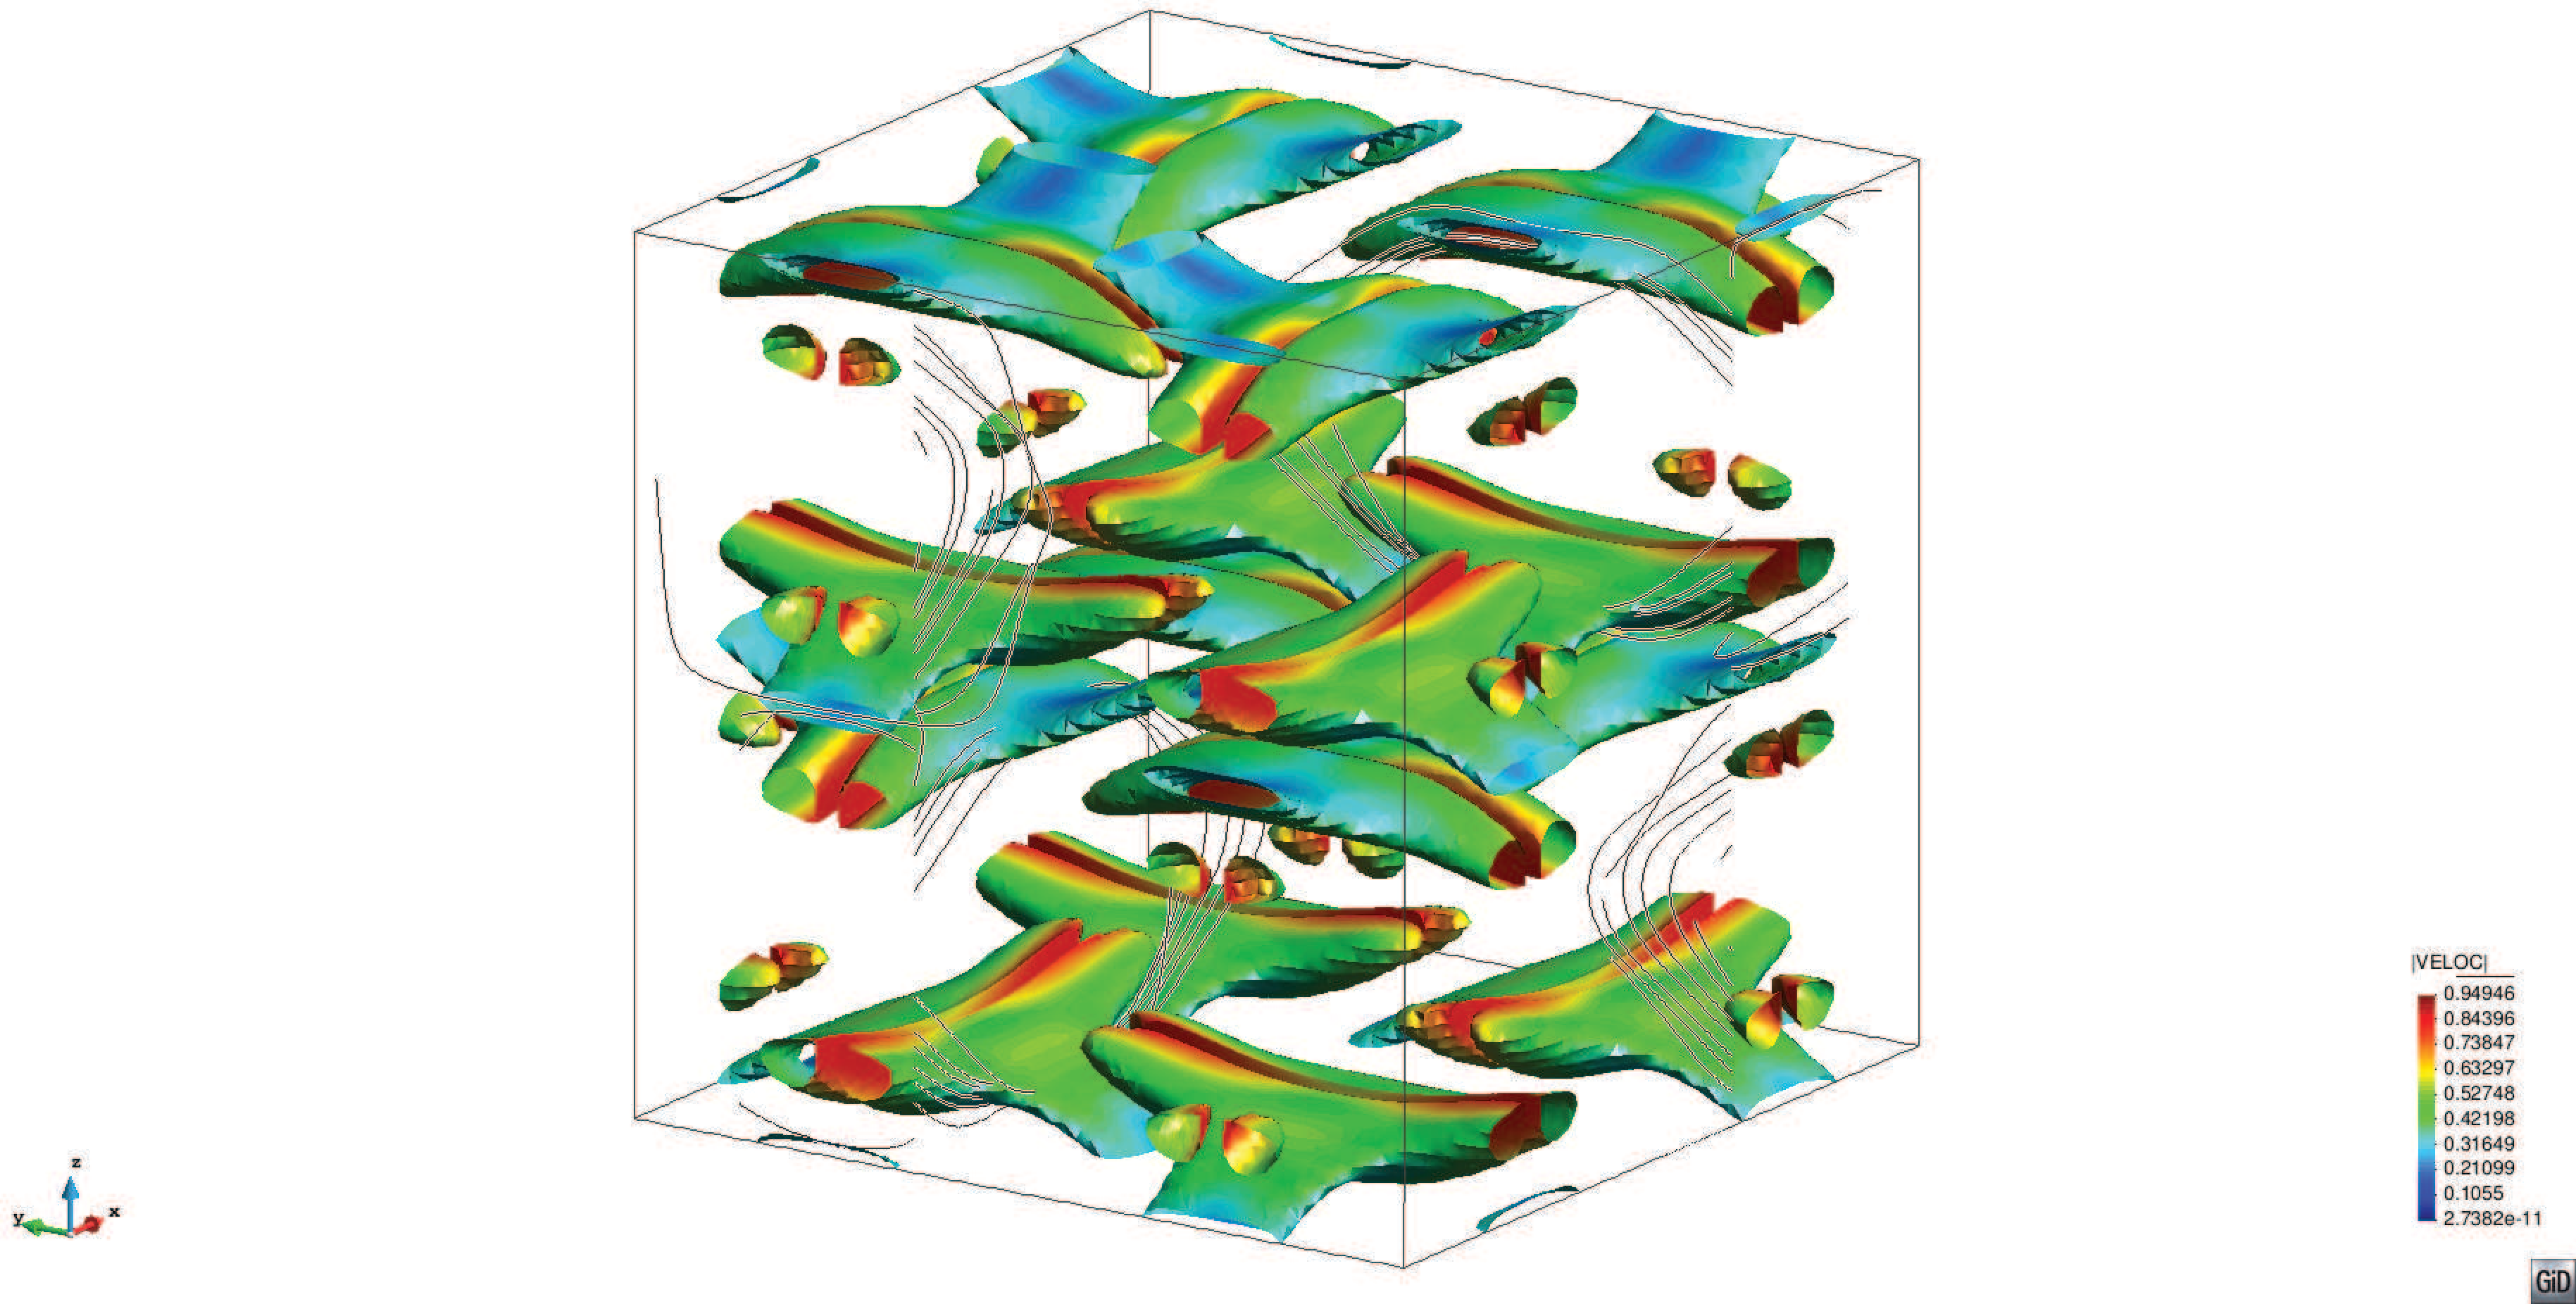
\includegraphics[clip=true, trim=13cm 0cm 13cm 0cm, width=0.6\textwidth]{Figures/Chapter3/TGV_isovorti_streaml_veloc_1}
	\caption{Vorticity isosurfaces at $t=4,0$ with streamlines for the TGV test.}
	\label{fig-TGV_vorticity_streamlines}
\end{figure}

\section{Turbulence in wall-bounded flow}
\label{sec-C3_wall_bounded}
The vast majority of turbulent flows that we can find in the nature are bounded by, at least, one solid surface. Some examples of bounded flows can be the flow throug a pipe or a duct, the flow in a channel or a river, the flow around an aircraft or a ship, or even the atmospheric flow that is bounded by the terrain. In a turbulent wall-bounded flow, the turbulence is generated through the viscous forces near the wall and then propagated to the outer layer. In this kind of flows, we are interested on defining the mean velocity profiles as well as the friction laws, which will allow us to determine the forces that the fluid flow exerts on the the solid wall.
\subsection{Mean flow}
\subsubsection{Shear stress}
Let us assume that within a certain region near the wall the mean velocity is parallel, or almost parallel, to that wall. We consider that we have a wall on the plane $ (x-z) $ where the mean flow is predominantly in the $ x $-direction, which we will denote as the stream-wise direction and statistically independent of $ z $. The $ y $-direction will be denoted by the wall-normal direction and the $ z $-direction the span-wise direction. Under this assumtions, $ \left\langle u_z\right\rangle=0 $ and the $ \left\langle u_x\right\rangle $ is independent of $ x $, leading to a mean continuity equation
\begin{equation}
\label{eq-mean_continuity}
\frac{d\left\langle u_y\right\rangle}{dy}=0.
\end{equation}

From the mean meomentum equation in the wall-normal direction we can conclude that the pressure is uniform across the flow, satisfying $$ \frac{\partial\left\langle p\right\rangle}{\partial x}=\frac{d p_w}{dx}, $$ being $ p_w(x) $ the pressure value at the wall. Then, from the axial mean momentum equation we have that the shear total shear stress $ \tau(y) $ follows
\begin{equation}
\label{eq-shear_stress_law}
\frac{d\tau}{dy}=\frac{d p_w}{dx},
\end{equation}
with
\begin{equation}
\label{eq-shear_stress}
\tau(y):=\nu\frac{d\left\langle u_x\right\rangle}{dy}-\left\langle u_xu_y\right\rangle,
\end{equation}
see \cite{pope} for a more detailed deduction. We will denote the wall shear stress as $ \tau_w:=\tau(0) $. It is seen that the shear stress is the sum of the viscous stress, $ \nu\frac{d\left\langle u_x\right\rangle}{dy} $, and the Reynolds stress $ -\left\langle u_xu_y\right\rangle $. At the wall, the no-slip boundary condition, $ \u=0 $, implies that
\begin{equation}
\label{eq-wall_shear_stress}
\tau_w=\nu\left.\frac{d\left\langle u_x\right\rangle}{dy}\right|_{y=0}.
\end{equation}

\subsubsection{Friction quantities}
From \Eq{wall_shear_stress} one can observe that the viscosity $ \nu $ is an important parameter in tubulent wall-bounded flows, particularly in the region near the wall. Hence, the mean velocity profile  will depend on the Reynolds number. Moreover, in the region near the wall we can define the appropiate viscous velocity and length scales. We will call friction velocity the velocity scale in the near-wall region, which is defined as
\begin{equation}
\label{eq-friction_velocity}
u_\tau:=\sqrt{\frac{\tau_w}{\rho}},
\end{equation}
and the viscous length scale as 
\begin{equation}
\label{eq-viscous_lenghtscale}
\delta_\nu:=\nu\sqrt{\frac{\rho}{\tau_w}}=\frac{\nu}{u_\tau}.
\end{equation}
Note that the Reynolds number based on the viscous scales is equal to the unity, $ Re_\nu = \frac{u_\tau\delta_\nu}{\nu}=1 $. An alternative is the so called friction Reynolds number, which is defined as
\begin{equation}
\label{eq-friction_reynolds}
Re_\tau:=\frac{u_\tau\delta}{\nu},
\end{equation}
being $ \delta $ the boundary layer thicknes. 

For wall-bounded turbulent flows it is a common practise to use the quantities in terms of wall units. We will define the distance from the wall in wall units as $ y^+:=\frac{y}{\delta_\nu}=\frac{u_\tau y}{\nu} $, and the mean stream-wise velocity in wall units as $ u^+:=\frac{\left\langle u_x\right\rangle}{u_\tau} $.

\subsubsection{Velocity profile}
It has been shown that in the region near the wall, the mean stream-wise velocity can be defined by the distance to the wall. This is known as the law of the wall, which can be expressed in wall units as $ u^+=f_w(y^+) $. In the inner layer, where $ y/\delta\le0.1 $, the law of the wall has been shown to follow the following expression
\begin{equation}
\label{eq-wall_law}
u^+=\frac{1}{\kappa}\ln y^++B,
\end{equation}
whith $ \kappa=0.41 $ and $ B=5.2 $.

\subsection{Benchmark tests}
\subsubsection{Turbulent Channel Flow}
\subsubsection{Turbulent Flow around an airfoil}

\section{Conclusions}
\label{sec-C3_conclusions}

blablabla...
